\documentclass[a4paper,12pt,oneside]{book}

%-------------------------------Start of the Preable------------------------------------------------
\usepackage[english]{babel}
\usepackage{blindtext}
%packagr for hyperlinks
\usepackage{hyperref}
\usepackage{float}
\hypersetup{
    colorlinks=true,
    linkcolor=blue,
    filecolor=magenta,      
    urlcolor=cyan,
}

\urlstyle{same}
%use of package fancy header
\usepackage{fancyhdr}
\setlength\headheight{26pt}
\fancyhf{}
%\rhead{
\includegraphics[width=1cm]{logo}}
\lhead{\rightmark}
\rhead{
\includegraphics[width=1cm]{logo}}
\fancyfoot[RE, RO]{\thepage}
\fancyfoot[CE, CO]{\href{http://www.e-yantra.org}{www.e-yantra.org}}

\pagestyle{fancy}

%use of package for section title formatting
\usepackage{titlesec}
\titleformat{\chapter}
  {\Large\bfseries} % format
  {}                % label
  {0pt}             % sep
  {\huge}           % before-code
 
%use of package tcolorbox for colorful textbox
\usepackage[most]{tcolorbox}
\tcbset{colback=cyan!5!white,colframe=cyan!75!black,halign title = flush center}

\newtcolorbox{mybox}[1]{colback=cyan!5!white,
colframe=cyan!75!black,fonttitle=\bfseries,
title=\textbf{\Large{#1}}}

%use of package marginnote for notes in margin
\usepackage{marginnote}

%use of packgage watermark for pages
%\usepackage{draftwatermark}
%\SetWatermarkText{
\includegraphics{logo}}
\usepackage[scale=2,opacity=0.1,angle=0]{background}
\backgroundsetup{
contents={
\includegraphics{logo}}
}

%use of newcommand for keywords color
\usepackage{xcolor}
\newcommand{\keyword}[1]{\textcolor{red}{\textbf{#1}}}

%package for inserting pictures
\usepackage{graphicx}

%package for highlighting
\usepackage{color,soul}

%new command for table
\newcommand{\head}[1]{\textnormal{\textbf{#1}}}


%----------------------End of the Preamble---------------------------------------


\begin{document}

%---------------------Title Page------------------------------------------------
\begin{titlepage}
\raggedright
{\Large eYSIP2016\\[1cm]}
{\Huge\scshape Autonomous Drone \\[.1in]}
\vfill
\begin{flushright}
{\large Akshit Gandhi \\}
{\large Keyur Rakholiya \\}
{\large Mentors: \\}
{\large Pushkar Raj\\}
{\large Akshat Jain \\}
{\large Rama Kumar \\}
{\large Duration of Internship: $ 21/05/2016-10/07/2016 $ \\}
\end{flushright}

{\itshape 2016, e-Yantra Publication}
\end{titlepage}
%-------------------------------------------------------------------------------

\chapter[Project Tag]{Autonomous Drone}
\section*{Abstract}
The latest innovation in the aviation industry is the Drone Technology. But, the drones that require manual input are very susceptible to radio interference or radio connection losses which can lead to disastrous results with your drone, such as crashes, etc. So, we came up with a solution, the solution is to make it \textbf{Autonomous!} i.e no manual input. 
\paragraph{}The drone has a companion computer on-board (Raspberry Pi) which guides the drone. These kind of drones can be used for security & surveillance, perimeter defense, mapping unreachable or hard to reach sites and even archaeological sites!, aerial photography, military purposes, forest survey, etc.
\paragraph{} So, as far as the project is concerned the drone we have designed has the following key features.
    \begin{itemize}
      \item Autonomous Take-off and Land
      \item Manual control using keyboard via remote login with Raspberry Pi
      \item Autonomous Take-off and Land (indoors) with ultrasonic sensors
      \item Autonomous flight between multiple points
    \end{itemize}

\subsection*{Completion status}
The project has been \textbf{completed} successfully. The tasks which we have accomplished are noted below.
    \begin{enumerate}
        \item Calculations for deciding the components to be used for drone.
        \item Assembly of Drone.
        \item Calibrating APM.
        \item First Manual Test Flight.
        \item Interfacing GPS with APM and reading values from it.
        \item Interfacing Ultrasonic Sensor with APM and reading values from it.
        \item Setting up the Raspberry Pi.
        \item Create a Power distribution system for the drone, RPi and APM.
        \item \textbf{Interfacing the Raspberry Pi with APM.}
        \item Manual flight using Raspberry Pi (remote login).
        \item Auto take-off and landing using Raspberry Pi.
        \item Semi-Autonomous Flight.
        \item Completely Autonomous Flights.
    \end{enumerate}

\section{Hardware parts}
\begin{itemize}
  \item F450 Frame: \href{https://github.com/eYSIP-2016/Autonomous-Drone/blob/master/datasheets/F450.pdf}{Datasheet}, \href{http://www.amazon.in/Neewer-99035841-4-Axis-Airframe/dp/B00ATLP6WM?ie=UTF8&psc=1&redirect=true&ref_=oh_aui_detailpage_o02_s00}{Vendor link}.
  \item 30 A ESC (DYS): \href{https://github.com/eYSIP-2016/Autonomous-Drone/blob/master/datasheets/ESC.pdf}{Datasheet}.
  \item D2282 1100 Kv Brushless Motors (DYS): \href{https://github.com/eYSIP-2016/Autonomous-Drone/blob/master/datasheets/dys_D2822_motors.pdf}{Datasheet}.
  \item 10x4.5 Proppellers 2 Clockwise and 2 Counter-clockwise rotation.
  \item Anti-vibration mount for APM 2.6.
   \item Fly-Sky CT-6B Transmitter & Receiver for manual flight: \href{https://github.com/eYSIP-2016/Autonomous-Drone/blob/master/datasheets/Radio.pdf}{Datasheet}.
   \item Ardupilot flight controller v2.6: \href{https://github.com/eYSIP-2016/Autonomous-Drone/blob/master/datasheets/APM-2.6-web-version.pdf}{Datasheet}, \href{http://ardupilot.org/copter/index.html}{Official Documentation}
   \item Raspberry Pi B+: \href{https://github.com/eYSIP-2016/Autonomous-Drone/blob/master/datasheets/raspberry%20pi%20B%2B.pdf}{Datasheet}.
   \item Lithium Polymer 3 Cell, 11.1V, 5000mAh, 20C discharge Battery: \href{http://www.nex-robotics.com/products/batteries-and-chargers/lithium-polymer-3-cell-11-1v-5000mah-20c-discharge-battery.html}{Datasheet and Vendor}.
   \item GPS Module: \href{https://github.com/eYSIP-2016/Autonomous-Drone/blob/master/datasheets/AqT_GNSS%20Patch%20Module%20user%20guide%20V1.0%20(1).pdf}{Datasheet}.
    \item Ultrasonic Sensor HC-SR04: \href{https://github.com/eYSIP-2016/Autonomous-Drone/blob/master/datasheets/HCSR04.pdf}{Datasheet}.
  \item Connection diagram
\end{itemize}

\section{Software used}
\begin{enumerate}
    \item Ardupilot Copter Firmware
        \paragraph{}This is a firmware for the APM 2.6 board.
        \begin{itemize}
          \item Detail of software: ACv3.2.1 and it can be downloaded from the mission planner itself or follow the \href{http://firmware.ardupilot.org/Copter/stable/apm2-quad/}{link}.
          \item To load the firmware follow the tutorials section of Autonomous Drone or follow this \href{https://github.com/eYSIP-2016/Autonomous-Drone/tree/master/Tutorials/Calibarting-APM}{link}
        \end{itemize}
  \item Mission Planner (Ground Station System)
    \paragraph{}\textbf{Details:} Mission Planner is a ground control station for Plane, Copter and Rover. It is compatible with Windows only. Mission Planner can be used as a configuration utility or as a dynamic control supplement for your autonomous vehicle.
        \begin{itemize}
          \item Load the firmware (the software) into the autopilot (APM, PX4...) that controls your vehicle.
          \item Setup, configure, and tune your vehicle for optimum performance.
          \item Plan, save and load autonomous missions into you autopilot with simple point-and-click way-point entry on Google or other maps.
          \item Download and analyze mission logs created by your autopilot.
          \item Interface with a PC flight simulator to create a full hardware-in-the-loop UAV simulator.
        
  \item Detail of software: \textbf{Version 1.3.30}, \href{http://firmware.ardupilot.org/Tools/MissionPlanner/MissionPlanner-latest.msi}{Download link}
  \item Installation steps:
    \begin{enumerate}
      \item Download the software from above link.
      \item Follow the detailed installtion procedure on \href{https://github.com/eYSIP-2016/Autonomous-Drone/blob/master/Tutorials/Calibarting-APM/Calibarting_the_APM-2.6.pdf}{this link} and also you can visit the documentation on \href{http://ardupilot.org/planner/docs/common-install-mission-planner.html}{this link}
    \end{enumerate}
  \end{itemize}
  \item MobaXterm (For SSH with Raspberry Pi)
    \paragraph{}\textbf{Details:}MobaXterm is your ultimate toolbox for remote computing. In a single Windows application, it provides loads of functions that are tailored for programmers, webmasters, IT administrators and pretty much all users who need to handle their remote jobs in a more simple fashion.
\paragraph{}
MobaXterm provides all the important remote network tools (SSH, X11, RDP, VNC, FTP, MOSH, ...) and Unix commands (bash, ls, cat, sed, grep, awk, rsync, ...) to Windows desktop, in a single portable exe file which works out of the box.
    \begin{itemize}
      \item Detail of software: Version 9.1 Home Edition, \href{http://mobaxterm.mobatek.net/download-home-edition.html}{Download link}
      \item Installation steps:
        \begin{enumerate}
          \item  Download MobaXterm from website link above.
          \item  Launch MobaXterm installer.
          \item Click Next to start installation. Accept the license agreement and click Next.
          \item Choose installation folder, then click Next. Then click Install.
          \item After the installation, click Finish.
          \item To create a session, Open MobaXterm
          \item Click Session to create a new session.
          \item Configure the new session for user root.
        \end{enumerate}
    \end{itemize}
\end{enumerate}

\section{Assembly of hardware}
	 \subsection{Assembly for manual flight}
	 \subsubsection{Assembling the Motors}
	 	Once you get the motors, the very first job is to mount the motors on the F450 frame. For this you will need M3 screws, so with the help of a screw-driver or L-key mount the motors on the arm of the quad like this:
	 	\begin{figure}[H]
	 	
	 	\centering
		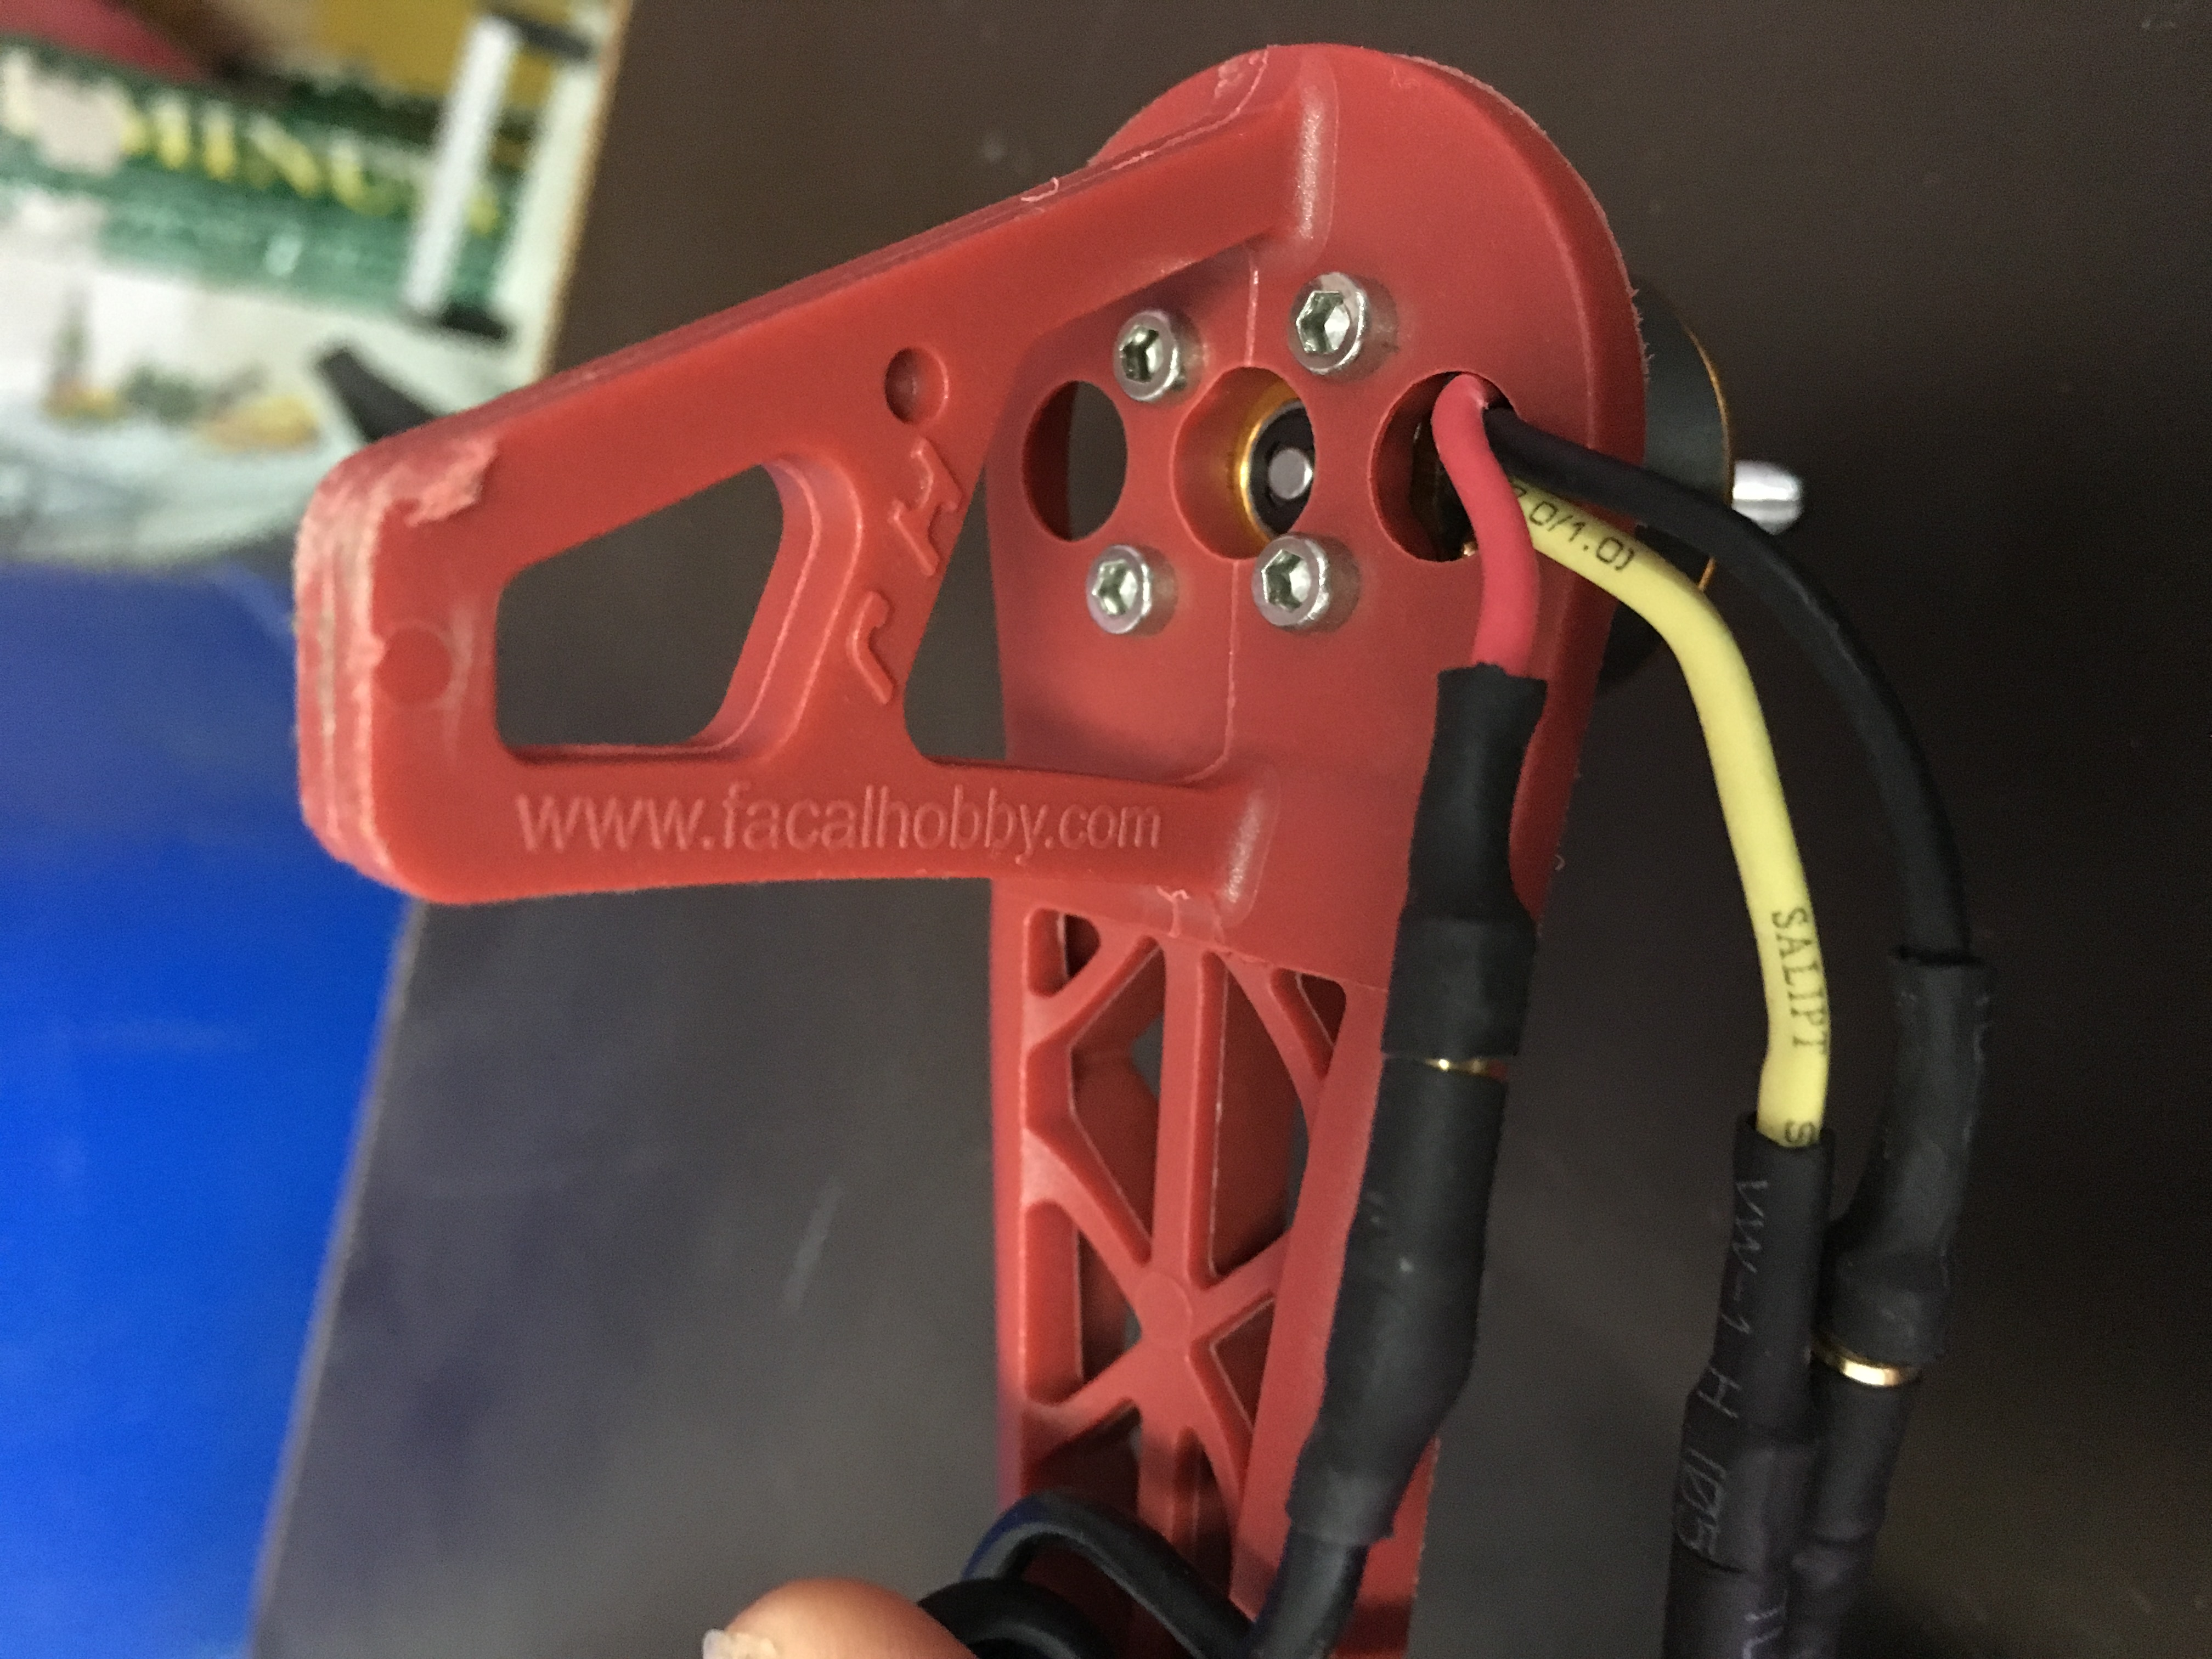
\includegraphics[width=5cm,height=5cm]{Screw}
		\caption{installing motors}
	 	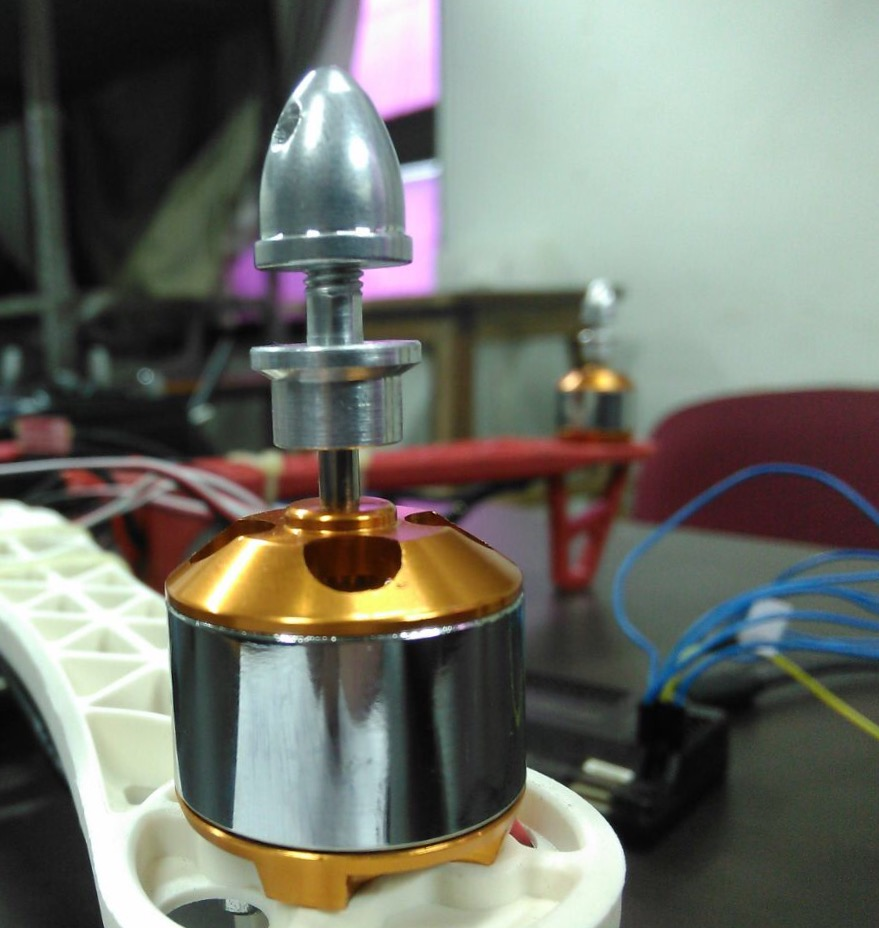
\includegraphics[width=5cm,height=5cm]{mot}
	 	\caption{Motor Assembly.}
\end{figure}
	 	\subsubsection{Esc mount}
	 	After the motors have been attached on the arms, next job is to attach the esc's, you can tie individual esc's on the arms using cable ties as shown below.
		 	
	 	 Also connect 3 wires from the esc's to the 3 wires on the motor, don't worry about the order in which the wires have to be connected we will look upon that in later tutorials.on ce your arms are ready with the escs and motors it will look something like this:
	 	 \begin{figure}[H]
	 	
	 	\centering
		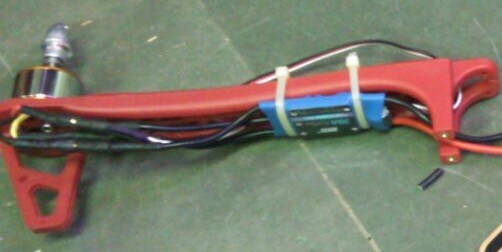
\includegraphics[width=10cm,height=5cm]{Esc}
		\caption{Esc Assembly.}
		\end{figure}
		
		\subsubsection{Connecting Esc to Power distribution board}
		The F450 frame comes with an inbuilt power distribution board so you just need to solder the esc wires (both positive and ground) to the pcb on the base plate. The pcb would look something like this.
		\begin{figure}[H]
	 	
	 	\centering
		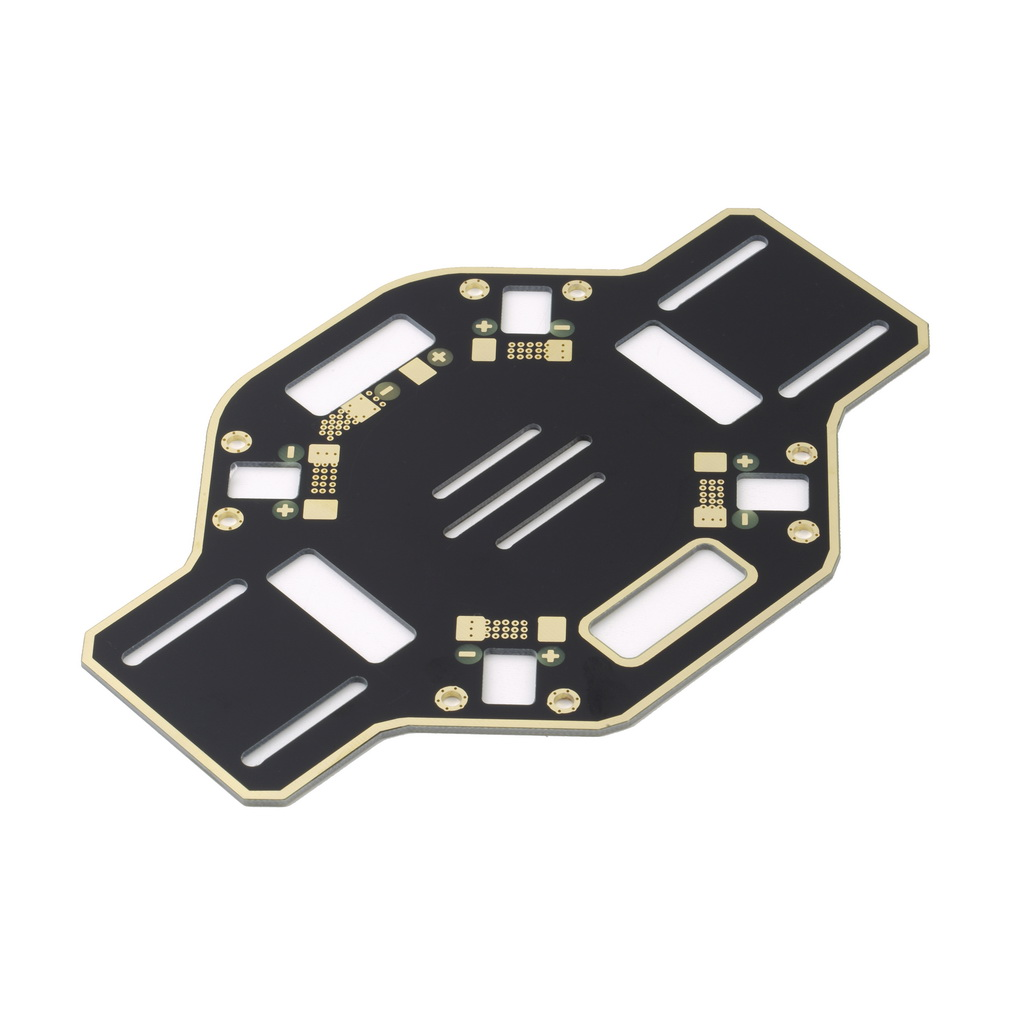
\includegraphics[width=7cm,height=7cm]{pcb}
		\caption{Power distribution Board.}
		\end{figure}
		
You will see that there are some points to attach the esc's marked as + or - and also on extra pair of points will be there for connecting the battery to the distribution board. First you need to ensure that there are no connectors on the esc( on the +ve and -ve wires), if there are any connectors desolder them and then solder the wires onto the pcb. Special care to ensure that +ve wires is soldered onto the +ve of the pcb and respectively for negative. Once you have soldered the wires onto the assembly would look something like this:
		\begin{figure}[H]
	 	
	 	\centering
		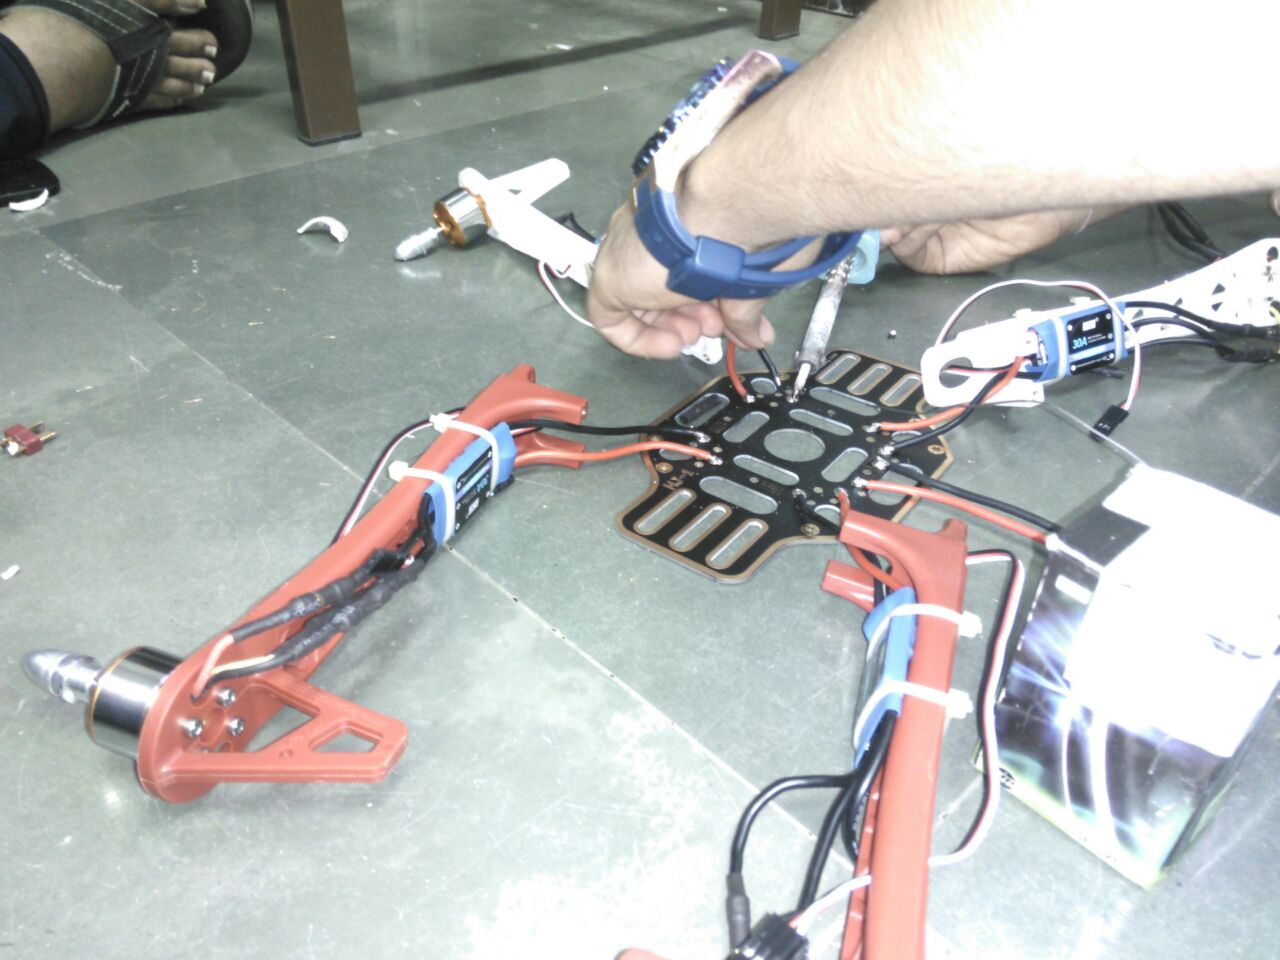
\includegraphics[width=12cm,height=6.5cm]{solder}
		\caption{Soldering.}
		\end{figure}
		
		\begin{figure}[H]
	 	
	 	\centering
		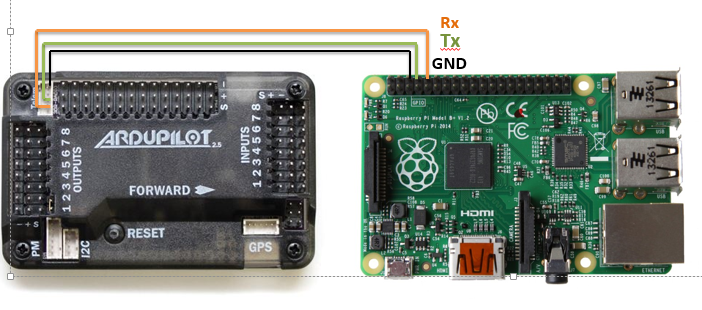
\includegraphics[width=12cm,height=6.5cm]{apmtopi}
		\caption{APM connected with R-pi}
		\end{figure}
		\begin{figure}[H]
		\centering
		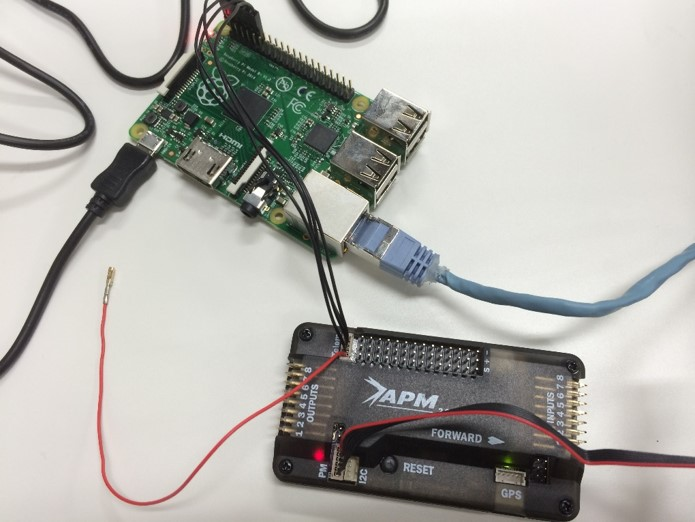
\includegraphics[width=12cm,height=6.5cm]{photo}
		\caption{Wiring Schematic.}
		\end{figure}
		
		\subsubsection{Assembling the frame together}
		Now you have your frame ready the next step is to use the screws provided with the kit to mount the arms on the lower plate and after that attach the upper plate. After this step your quad should look like this:
		\paragraph{}But an IMPORTANT note: To make it easy for you to know the orientation of the quad you can setup the frame in such a way that 2 adjacent white/red arms point to the forward direction of the quad.
		\begin{figure}[H]
	 	
	 	\centering
		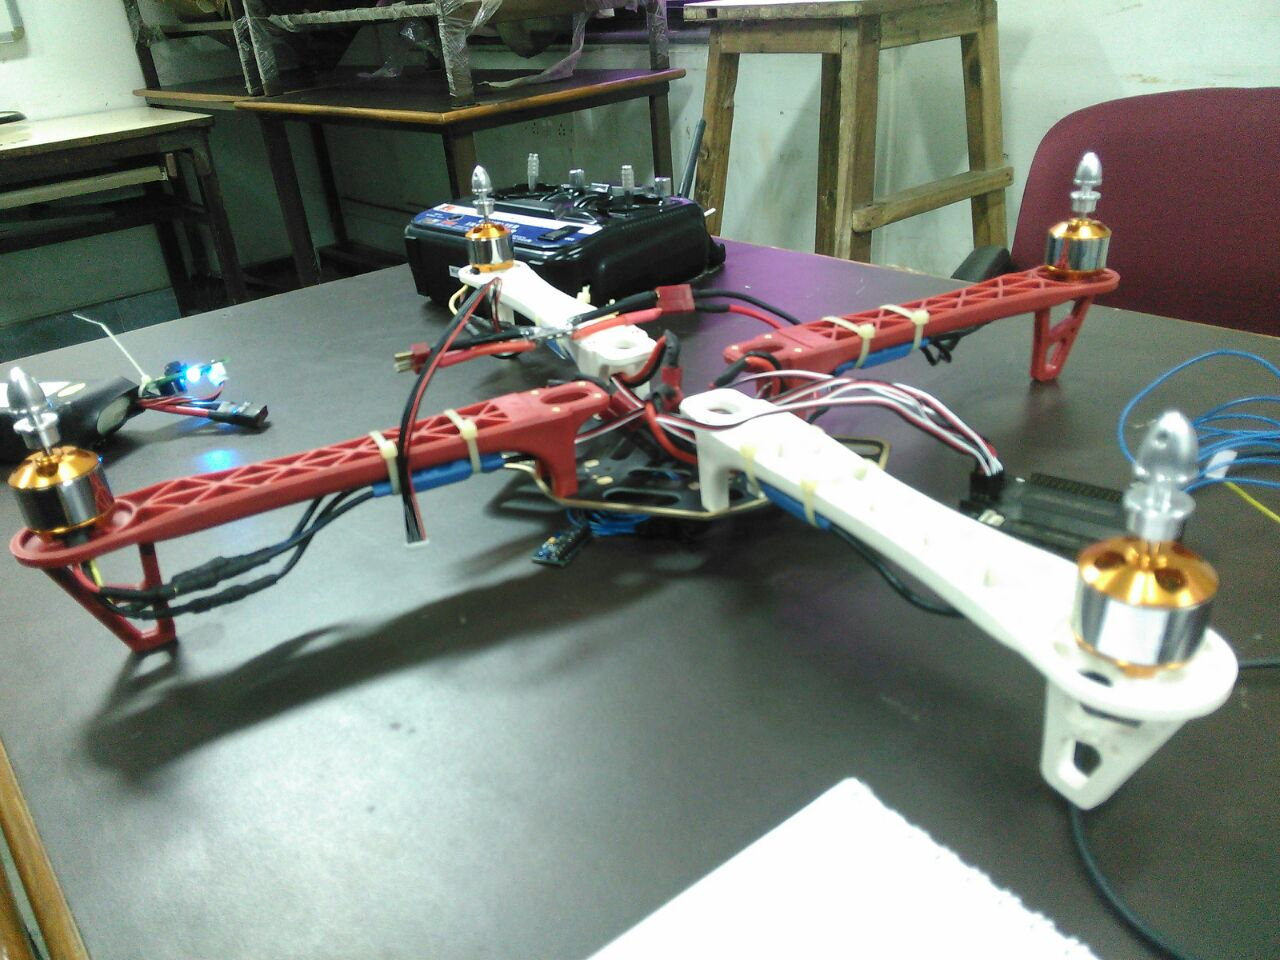
\includegraphics[width=12cm,height=7cm]{Frame}
		\caption{Frame Assembly w/o upper plate mounted.}
		\end{figure}
		
		\subsubsection{Mounting your Flight Controller}
		For the autonomous drone application we are usin APM 2.6 as our flight controller, but you can use any flight controller of your choice like KK 2.x board, CC3D, Naze 32, Pixhawk, KISS,etc. The basic step to mount any flight controller on the deck of the frame is by mounting it by using an anti-vibration mount. Using it is very important as it reduces the amount of vibrations that reach the controller. As unwanted vibrations can lead to erroneous results.
		\paragraph{}So were are using the antivibration mount for the APM. So depending on your flight controller you can mount it on the mount by using double sided tapes. But before mounting the vibration mount on the deck ensure that the forward direction of the FC matches with the forward direction of your quad decided by you.
		
		\subsubsection{Wiring the flight controller}
		Now depending on your flight controller you have to wire up your Flight controller with the receiver and the ESC's. Here we will demonstrate the connections for the APM 2.6 .
		\paragraph{} Another important note is to make the motor connections properly i.e. the first motor connects to port 1 on the APM and son on. The below pictures will make it very clear.
		\begin{figure}[H]
	 	\centering
		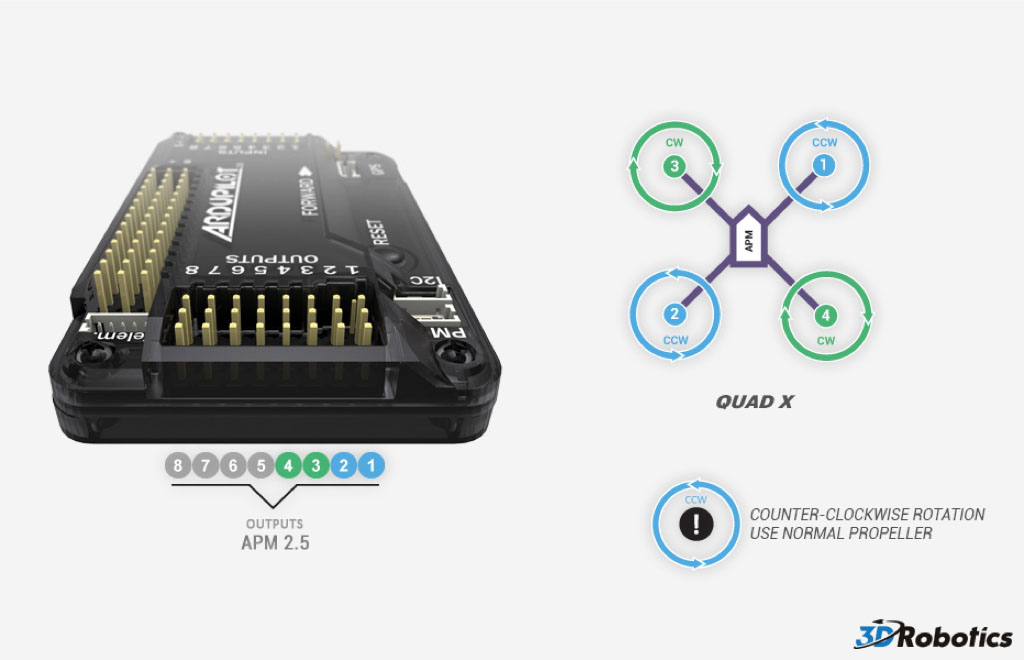
\includegraphics[width=12cm,height=7cm]{direction}
		\caption{Motor Layout For quad X config.}
		\end{figure}
		\paragraph{}Don't worry about the motor spin direction we will solve it in a moment. Now let's see how to make connections with the APM. Refer the below figure. Don't bother about the GPS and Gimbal, they are just extra accessories.
		\begin{figure}[H]
    \begin{center}
    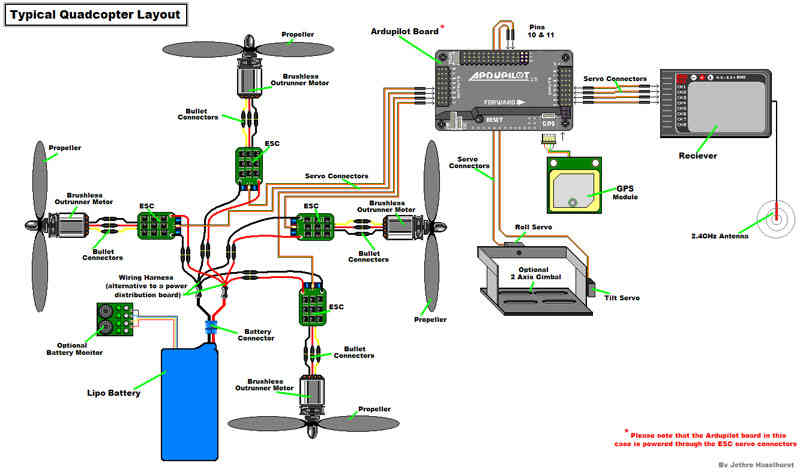
\includegraphics[scale=0.6]{APM}
    \caption{APM wiring}
    \label{fig: figure}
    \end{center}
\end{figure}
	\paragraph{•}
	Now if you have followed the above steps properly, you are ready for the calibration of your flight controller. Now here we are done with the assembly.
	
	\paragraph{}\textbf{Note:} for calibration of APM refer to the tutorials on autonomous drone repository on this \href{https://github.com/eYSIP-2016/Autonomous-Drone/tree/master/Tutorials/Calibarting-APM}{link}
\subsection{Assembly for Autonomous flight}
This section explains how to connect and configure a Raspberry Pi (RPi) so that it is able to communicate with a APM flight controller using the MAVLink protocol\textbf{[2]} over a serial connection
	 \begin{figure}[H]
	 	\centering
		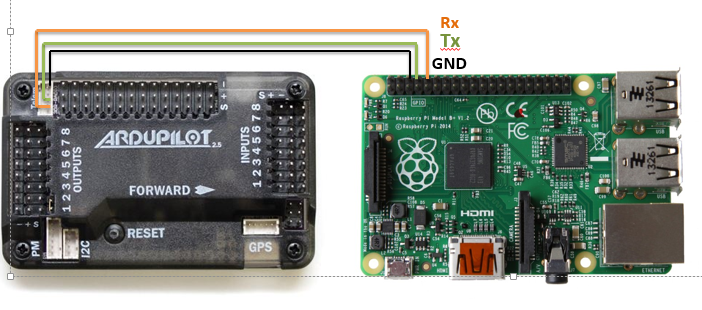
\includegraphics[scale=0.35]{apmtopi}
	 	\caption{Connection diagram.}
\end{figure}
	\paragraph{•} The picture shown above is for pixhawk controller but the same connection works for APM also.
	 \subsubsection{Connecting to RPi with an SSH/Telnet client}
	 \textbf{NOTE:} These steps assume that you have already set-up your RPi so that it is running Raspbian.

To avoid the requirement to plug a keyboard, mouse and HDMI screen into your RPi it is convenient to be able to connect from your Desktop/Laptop computer to your RPi using an SSH/Telnet client such as PuTTY.
	 \begin{itemize}
	 	\item Connect the RPi to your local network by one of the following methods:
			\begin{itemize}
				\item Connecting an Ethernet LAN cable from the RPi board to your Ethernet router, or
				\item Use a USB dongle to connect your RPi to the local wireless network, or
				\item Connect the Ethernet LAN cable between the RPi and your desktop/laptop computer. Open the control panel’s Network and Sharing Center, click on the network connection through which your desktop/laptop is connected to the internet, select properties and then in the sharing tab, select “Allow other networks to connect through this computer’s Internet connection”
\end{itemize}
	\item Determine the RPi’s IP address:
	\begin{itemize}
		\item If you have access to the RPi’s terminal screen (i.e.you have a screen, keyboard, mouse connected) you can use the /sbin/ifconfig command.
			\begin{figure}[H]
				\centering
				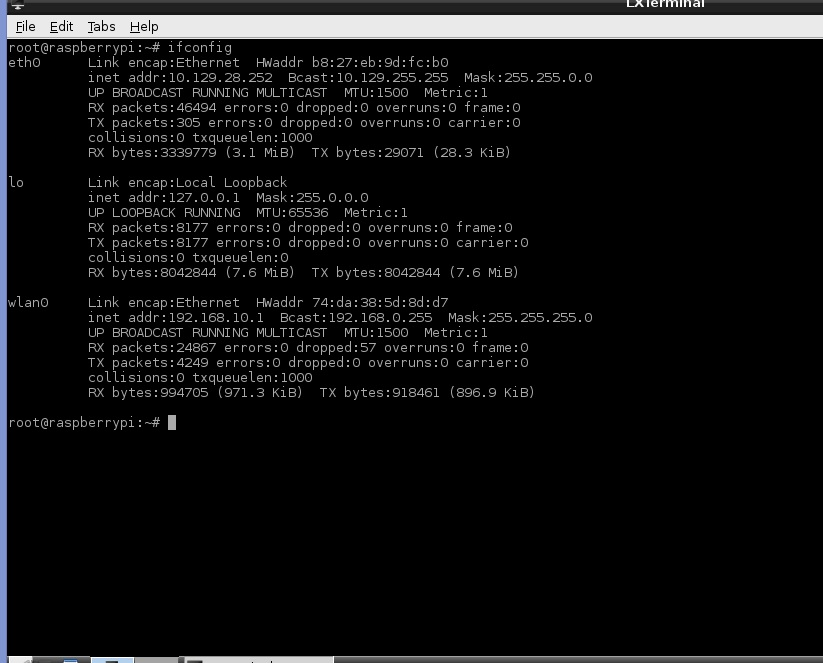
\includegraphics[scale=0.37]{ip}
				\caption{IP address on terminal.}
			\end{figure}
		\item If your Ethernet router has a web interface it may show you the IP address of all connected devices
	\end{itemize}	\item Connect with Putty:
		\begin{figure}[H]
	 	\centering
		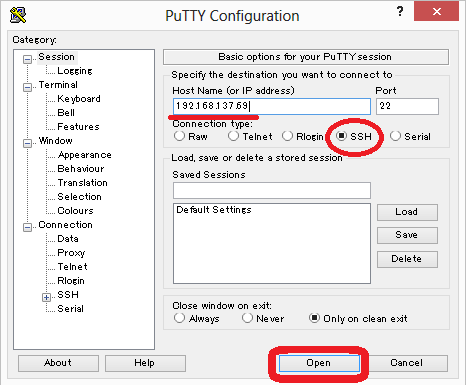
\includegraphics[scale=0.37]{putty}
	 	\caption{Connect screen with Putty.}
\end{figure}
	If all goes well you should be presented with the regular login prompt to which you can enter the username/password which defaults to pi/raspberry
	 \end{itemize}
	 \subsubsection{Install the required packages on the Raspberry Pi}
	 Log into the RPi board (default username password is pi/raspberry) and check that its connection to the internet is working. If there's some problem then troubleshooting guide can be found on the documentation site \url{http://ardupilot.org/dev/docs/raspberry-pi-via-mavlink.html}
	 \paragraph{After the internet connection is confirmed to be working install these packages:}
	 \begin{itemize}
	 	\item sudo apt-get update
	 	\item sudo apt-get install screen python-wxgtk2.8 python-matplotlib python-opencv python-pip python-numpy python-dev libxml2-dev libxslt-dev
	 	\item sudo pip install pymavlink
	 	\item sudo pip install mavproxy
	 \end{itemize}
	 \subsubsection{Disable the OS control of the serial port}
	 Use the Raspberry Pi configuration utility for this.
		\paragraph{}Type:
			\begin{itemize}
				\item sudo raspi-config
				\item And in the utility, select 								“Advanced Options”:
				\begin{figure}[H]
	 	\centering
		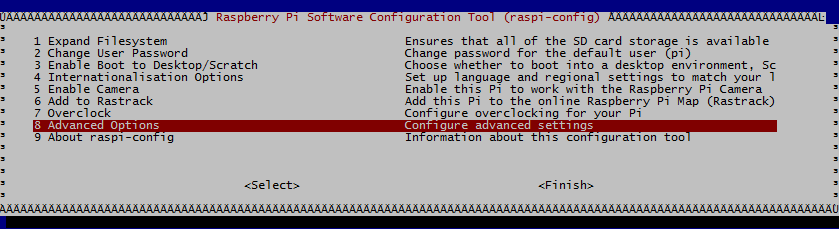
\includegraphics[scale=0.37]{adv1}
	 	\caption{RasPiConfiguration Utility: Serial Settings: Advanced Options.}
\end{figure}
		\begin{itemize}
			\item And then “Serial” to disable OS use of the serial connection:
			\begin{figure}[H]
	 	\centering
		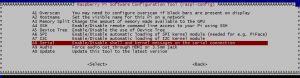
\includegraphics[scale=0.85]{adv2}
\end{figure}
		\end{itemize}
Reboot the Raspberry Pi when you are done.
			\end{itemize}
			\subsubsection{Testing the connection}
			To test the RPi and APM are able to communicate with each other first ensure the RPi and APM are powered, then in a console on the RPi type:
			\begin{itemize}
				\item sudo -s
				\item mavproxy.py --master=/dev/ttyAMA0 --baudrate 57600 --aircraft MyCopter
				
				raspberry pi's default port is connected with console input/output. so use this port we have to disable it first. now we have connected our device via UART port ot R-Pi. so "/dev/ttyAMA0" is a port for serial communication between R-pi and APM. 
				
				You configure BaudRate as bits per second. The transferred bits include the start bit, the data bits, the parity bit (if used), and the stop bits. However, only the data bits are stored.
				
				The baud rate is the rate at which information is transferred in a communication channel. In the serial port context, "9600 baud" means that the serial port is capable of transferring a maximum of 9600 bits per second. If the information unit is one baud (one bit), the bit rate and the baud rate are identical. If one baud is given as 10 bits, (for example, eight data bits plus two framing bits), the bit rate is still 9600 but the baud rate is 9600/10, or 960. You always configure BaudRate as bits per second. Therefore, in the previous example, set BaudRate to 9600.
				
				 
				Note: In the above command it's MyCopter and My-Copter
				\item Once MAVProxy has started you should be able to type in the following command to display the \texttt{ARMING\_CHECK} parameters value
				\begin{itemize}
					\item param show \texttt{ARMING\_CHECK}
					\item param set \texttt{ARMING\_CHECK} 0
					\item arm throttle
					\begin{itemize}
			\item And then “Serial” to disable OS use of the serial connection:
			\begin{figure}[H]
	 	\centering
		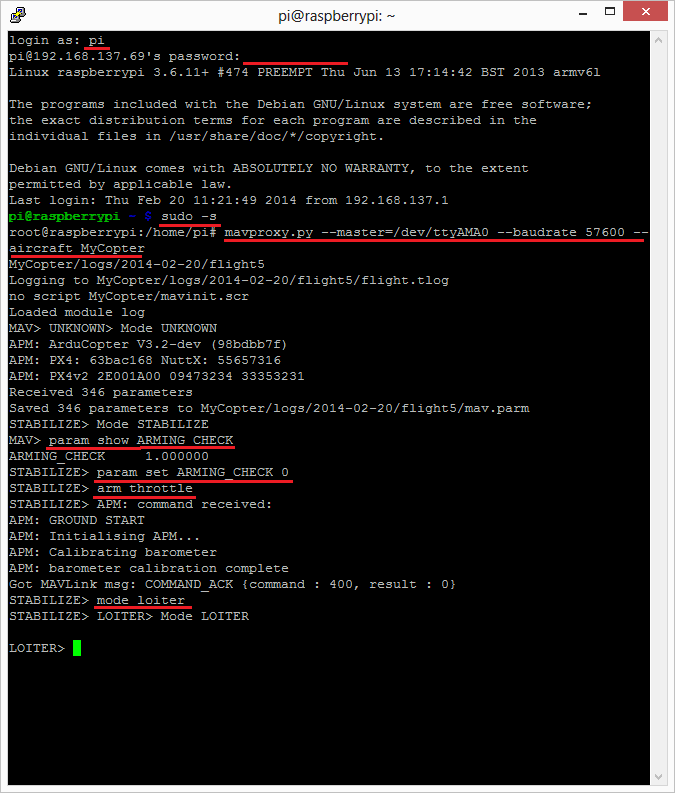
\includegraphics[scale=0.6]{connect}
		\caption{Terminal screen.}
\end{figure}
	\textbf{NOTE:} If you get an error about not being able to find log files or if this example otherwise doesn’t run properly, make sure that you haven’t accidentally assigned these files to another username, such as Root.
	\paragraph{•}Entering the following at the Linux command line will ensure that all files belong to the standard Pi login account:
	\item sudo chown -R pi /home/pi
		\end{itemize}
				\end{itemize}
				
			\end{itemize}
			\subsubsection{Configure MAVProxy to always run}
				To setup MAVProxy to start whenever the RPi is restarted open a terminal window and edit the /etc/rc.local file, adding the following lines just before the final “exit 0” line: 
				\begin{figure}[H]
	 	\centering
		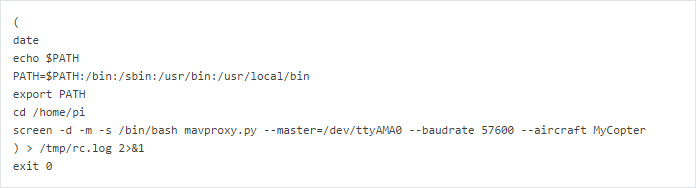
\includegraphics[scale=0.75]{command}
		
\end{figure}
\paragraph{To open /etc/rc.local file type in sudo nano /etc/rc.local and type the code below and save it in the file}
\paragraph{}If you wish to connect to the MAVProxy application that has been automatically started you can log into the RPi and type: sudo screen -x

\paragraph{}\textbf{Note:} For powering the Raspberry Pi from the drone refer \href{https://github.com/eYSIP-2016/Autonomous-Drone/blob/master/Tutorials/Power%20Management%20System/Powering_the_Set-Up.pdf}{this}.
\subsection{Interface GPS sensor with APM 2.6}
To connect the GPS to APM via GPS port which is given in APM.
		Follow this image for connections.
		\begin{figure}[H]

		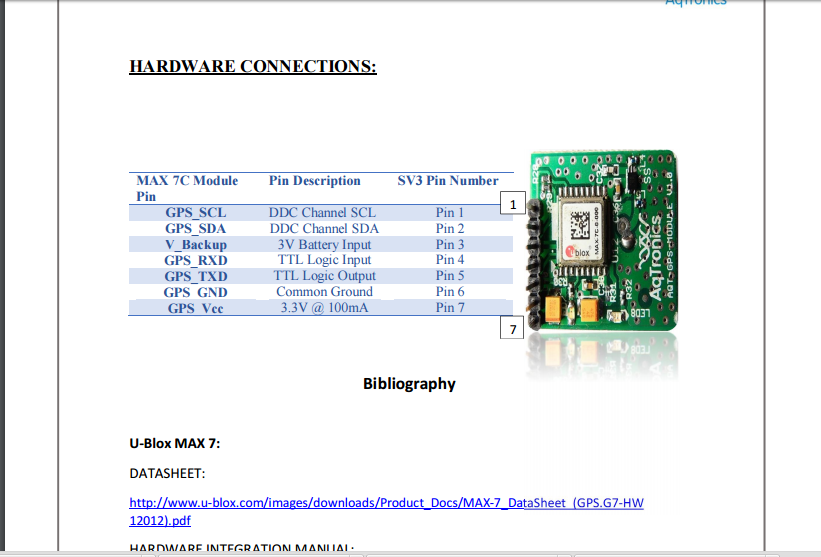
\includegraphics[width = 300px]{gps2}
			\caption{GPS module pin Diagram}
		
		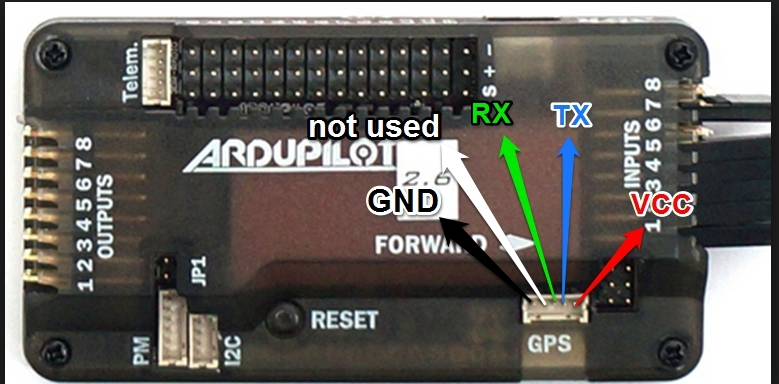
\includegraphics[width = 300px]{ardu2}
			\caption{GPS Pin on APM}
		\end{figure}
		connect the module as shown in figure. connect APM with Mission planner and go to under open sky.
		for perfect gps location you GPS module should be under open sky. after 2 or 3 minutes GPS satellites will be connected to module. and you will find your Location on map in MISSION PLANNER software. you can also see no. of satellites connected to your gps module. \\
		
		You will also get value of longitude,latitude,altitude on terminal of mission planner software.\newline
		
		\begin{figure}[H]
		\centering
		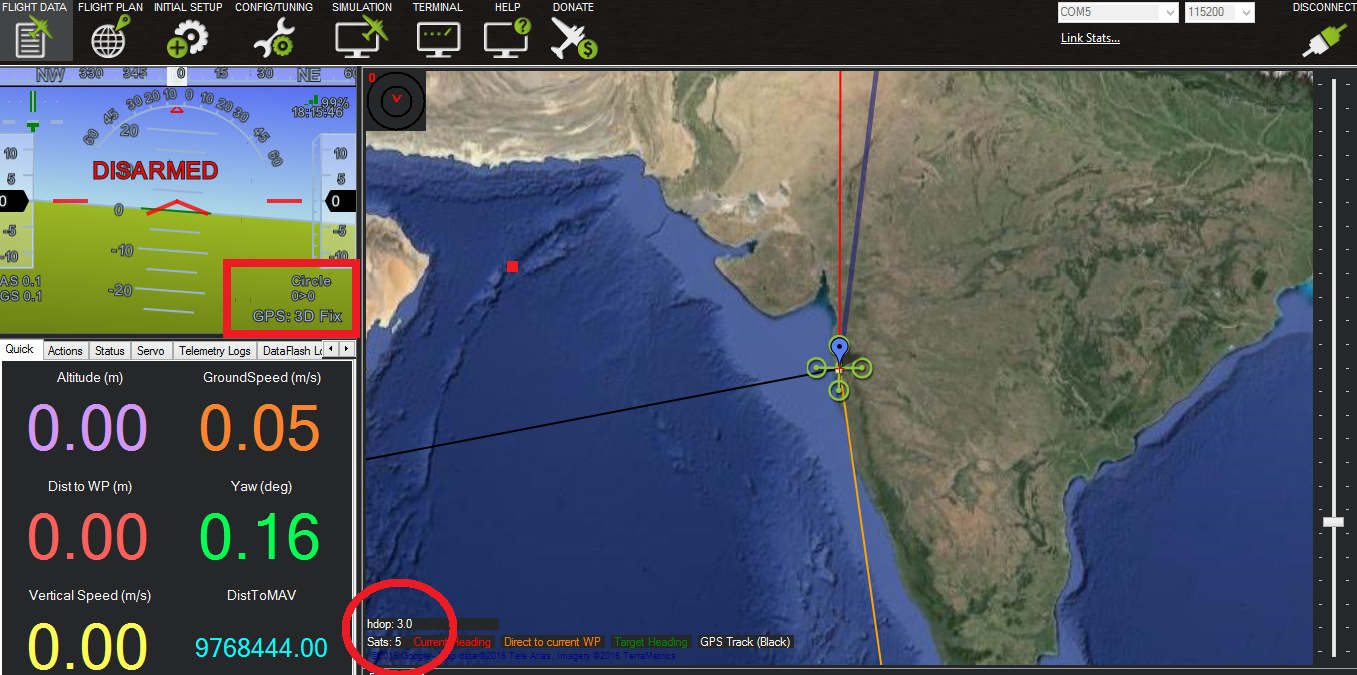
\includegraphics[width = 400px]{map1}
		\caption{Current location}
		\end{figure}
		As you can see in the figure. mission planner shows 3D fix and no. of satellites are 5.
		As you move from one place to another you will be tracked as you can see in image.
			\begin{figure}[H]
			    \centering
				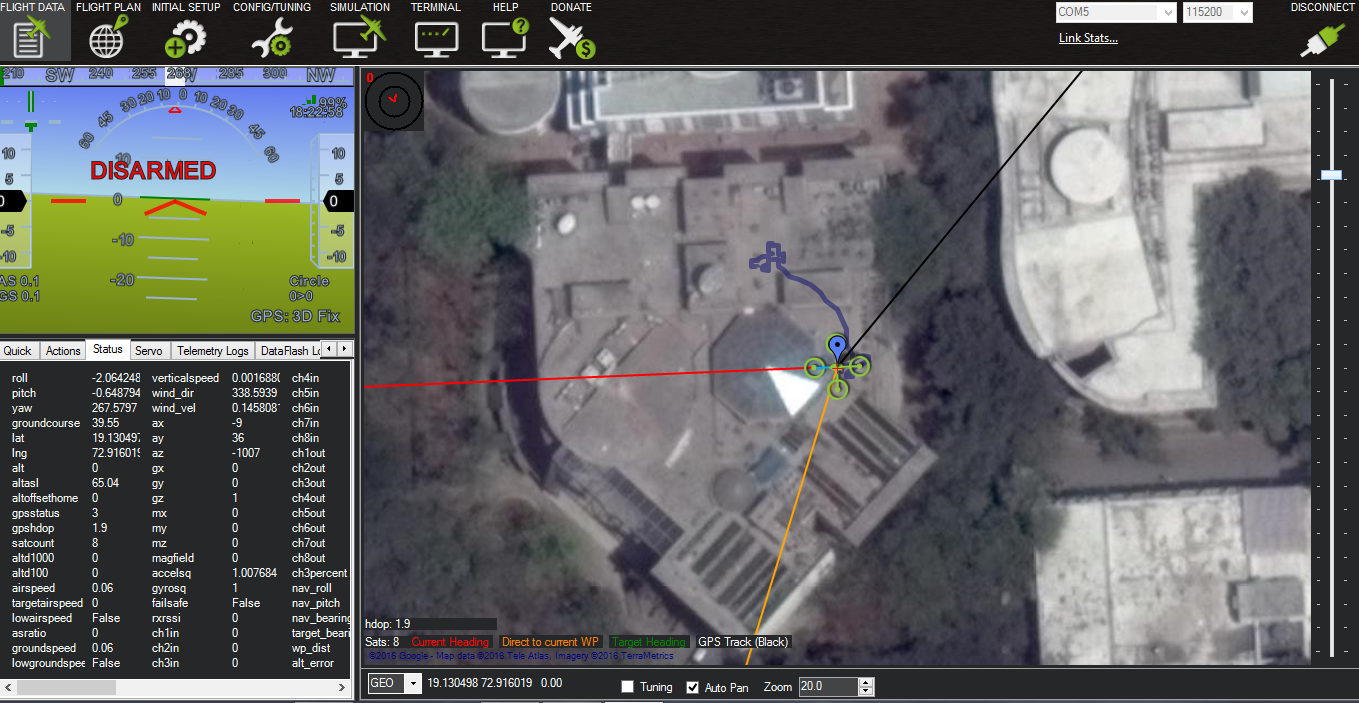
\includegraphics[width = 400px]{map2}
				\caption{Closer look to location}
			\end{figure}
	You can see  LAT , LON ,ALT and SATS on terminal.
		\begin{figure}[H]
		    \centering
			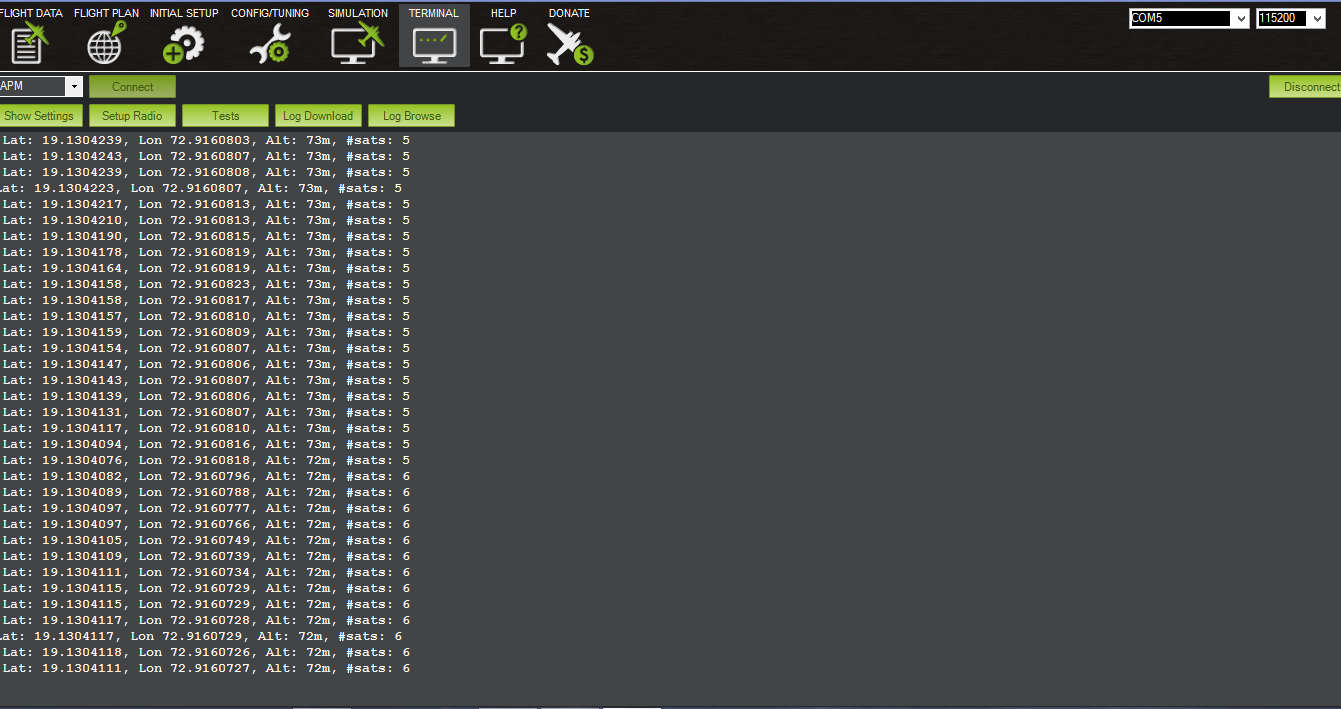
\includegraphics[width = 400px]{map3}
			\caption{DATA from terminal}
		\end{figure}

\subsection{Interface Ultrasonic sensor with Raspberry Pi}
\subsubsection{Connecting to R-Pi}
			Powering the module is easy. Just connect the +5V and Ground pins to Pin 2 and GPIO21 on the Pi’s GPIO header.
			\begin{figure}[h]
				\centering
				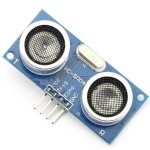
\includegraphics[scale=0.75]{sensor}
				\caption{HC-SR04 Sensor}
			\end{figure}

\paragraph{}The input pin on the module is called the “trigger” as it is used to trigger the sending of the ultrasonic pulse. Ideally it wants a 5V signal but it works just fine with a 3.3V signal from the GPIO. So we connected the trigger directly to GPIO20 on our GPIO header.
\paragraph{}
You can use any GPIO pins you like on your RPi but you will need to note the references and amend your Python script accordingly.
\paragraph{•}
The module’s output is called the “echo” and needs a bit more thought. The output pin is low (0V) until the module has taken its distance measurement. It then sets this pin high (+5V) for the same amount of time that it took the pulse to return. So our script needs to measure the time this pin stays high. The module uses a +5V level for a “high” but this is too high for the inputs on the GPIO header which only like 3.3V. In order to ensure the Pi only gets hit with 3.3V we can use a basic voltage divider. This is formed with two resistors.
\paragraph{•}
If R1 and R2 are the same then the voltage is split in half. This would give us 2.5V. If R2 is twice the value of R1 then we get 3.33V which is fine. So ideally you want R2 to be between R1 and R1 x 2. But we used 1000 and 680 ohm resistors (Because it worked the best for us!).
\paragraph{•}
Here is a diagram of our final circuit. We chose GPIO20 and GPIO16 [echo], but you can use any of the available GPIO pins on the GPIO header. Just remember to update the script.
	\begin{figure}[H]
	 	\centering
		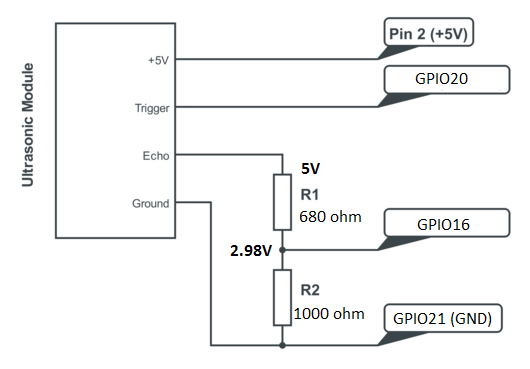
\includegraphics[width=7cm,height=5cm]{pin}
		\caption{Circuit Diagram}
	\end{figure}
	\subsubsection{Python Script}
		Once you have followed above connection diagram you can test the sensor you are ready with the next part i.e to access the sensor values using the python script. The script is in the codes folder.
	\subsubsection{Accuracy}
		\begin{itemize}
			\item The accuracy of the distance measurement is dependent on timing. Python under Linux is not ideal for precise timing but for general messing about it will work OK. To improve accuracy you would need to start looking at using C instead.
			\item When the GPIOs are configured the module needs some time before it is ready to take its first reading so we added a 0.5 second delay to the start of the script.
			\item The transducers have a wide angle of sensitivity. In a cluttered environment you may get shorter readings due to objects to the side of the module.
			\item Measurements work down to about 2cm. Below this limit the results can give strange results.
			\item If the ultrasonic transducers touch anything the results are unpredictable.
		\end{itemize}


\section{Software and Code}
\begin{enumerate}
  \item \href{https://github.com/eYSIP-2016/Autonomous-Drone/blob/master/code/Autonomus%20take%20off%20and%20landing.py}{Autonomous Takeoff and Landing}
  
  \item \href{https://github.com/eYSIP-2016/Autonomous-Drone/blob/master/code/Ultrasonic%20sensor%20take%20off.py}{Ultrasonic sensor take off}
  
  \item \href{https://github.com/eYSIP-2016/Autonomous-Drone/blob/master/code/quad%20control%20with%20keyboard.py}{Quadcopter using keyboard control}
  
  \item \href{https://github.com/eYSIP-2016/Autonomous-Drone/blob/master/code/A_to_B%20point%20Autonomous.py}{A to B point Autonomous}
\end{enumerate}
 

Brief explanation of various parts of code is given in comments of code.
\newpage
\section{Use and Demo}

    \textbf{Actual Drone Images}
    \begin{figure}[H]
        \centering
        \fbox{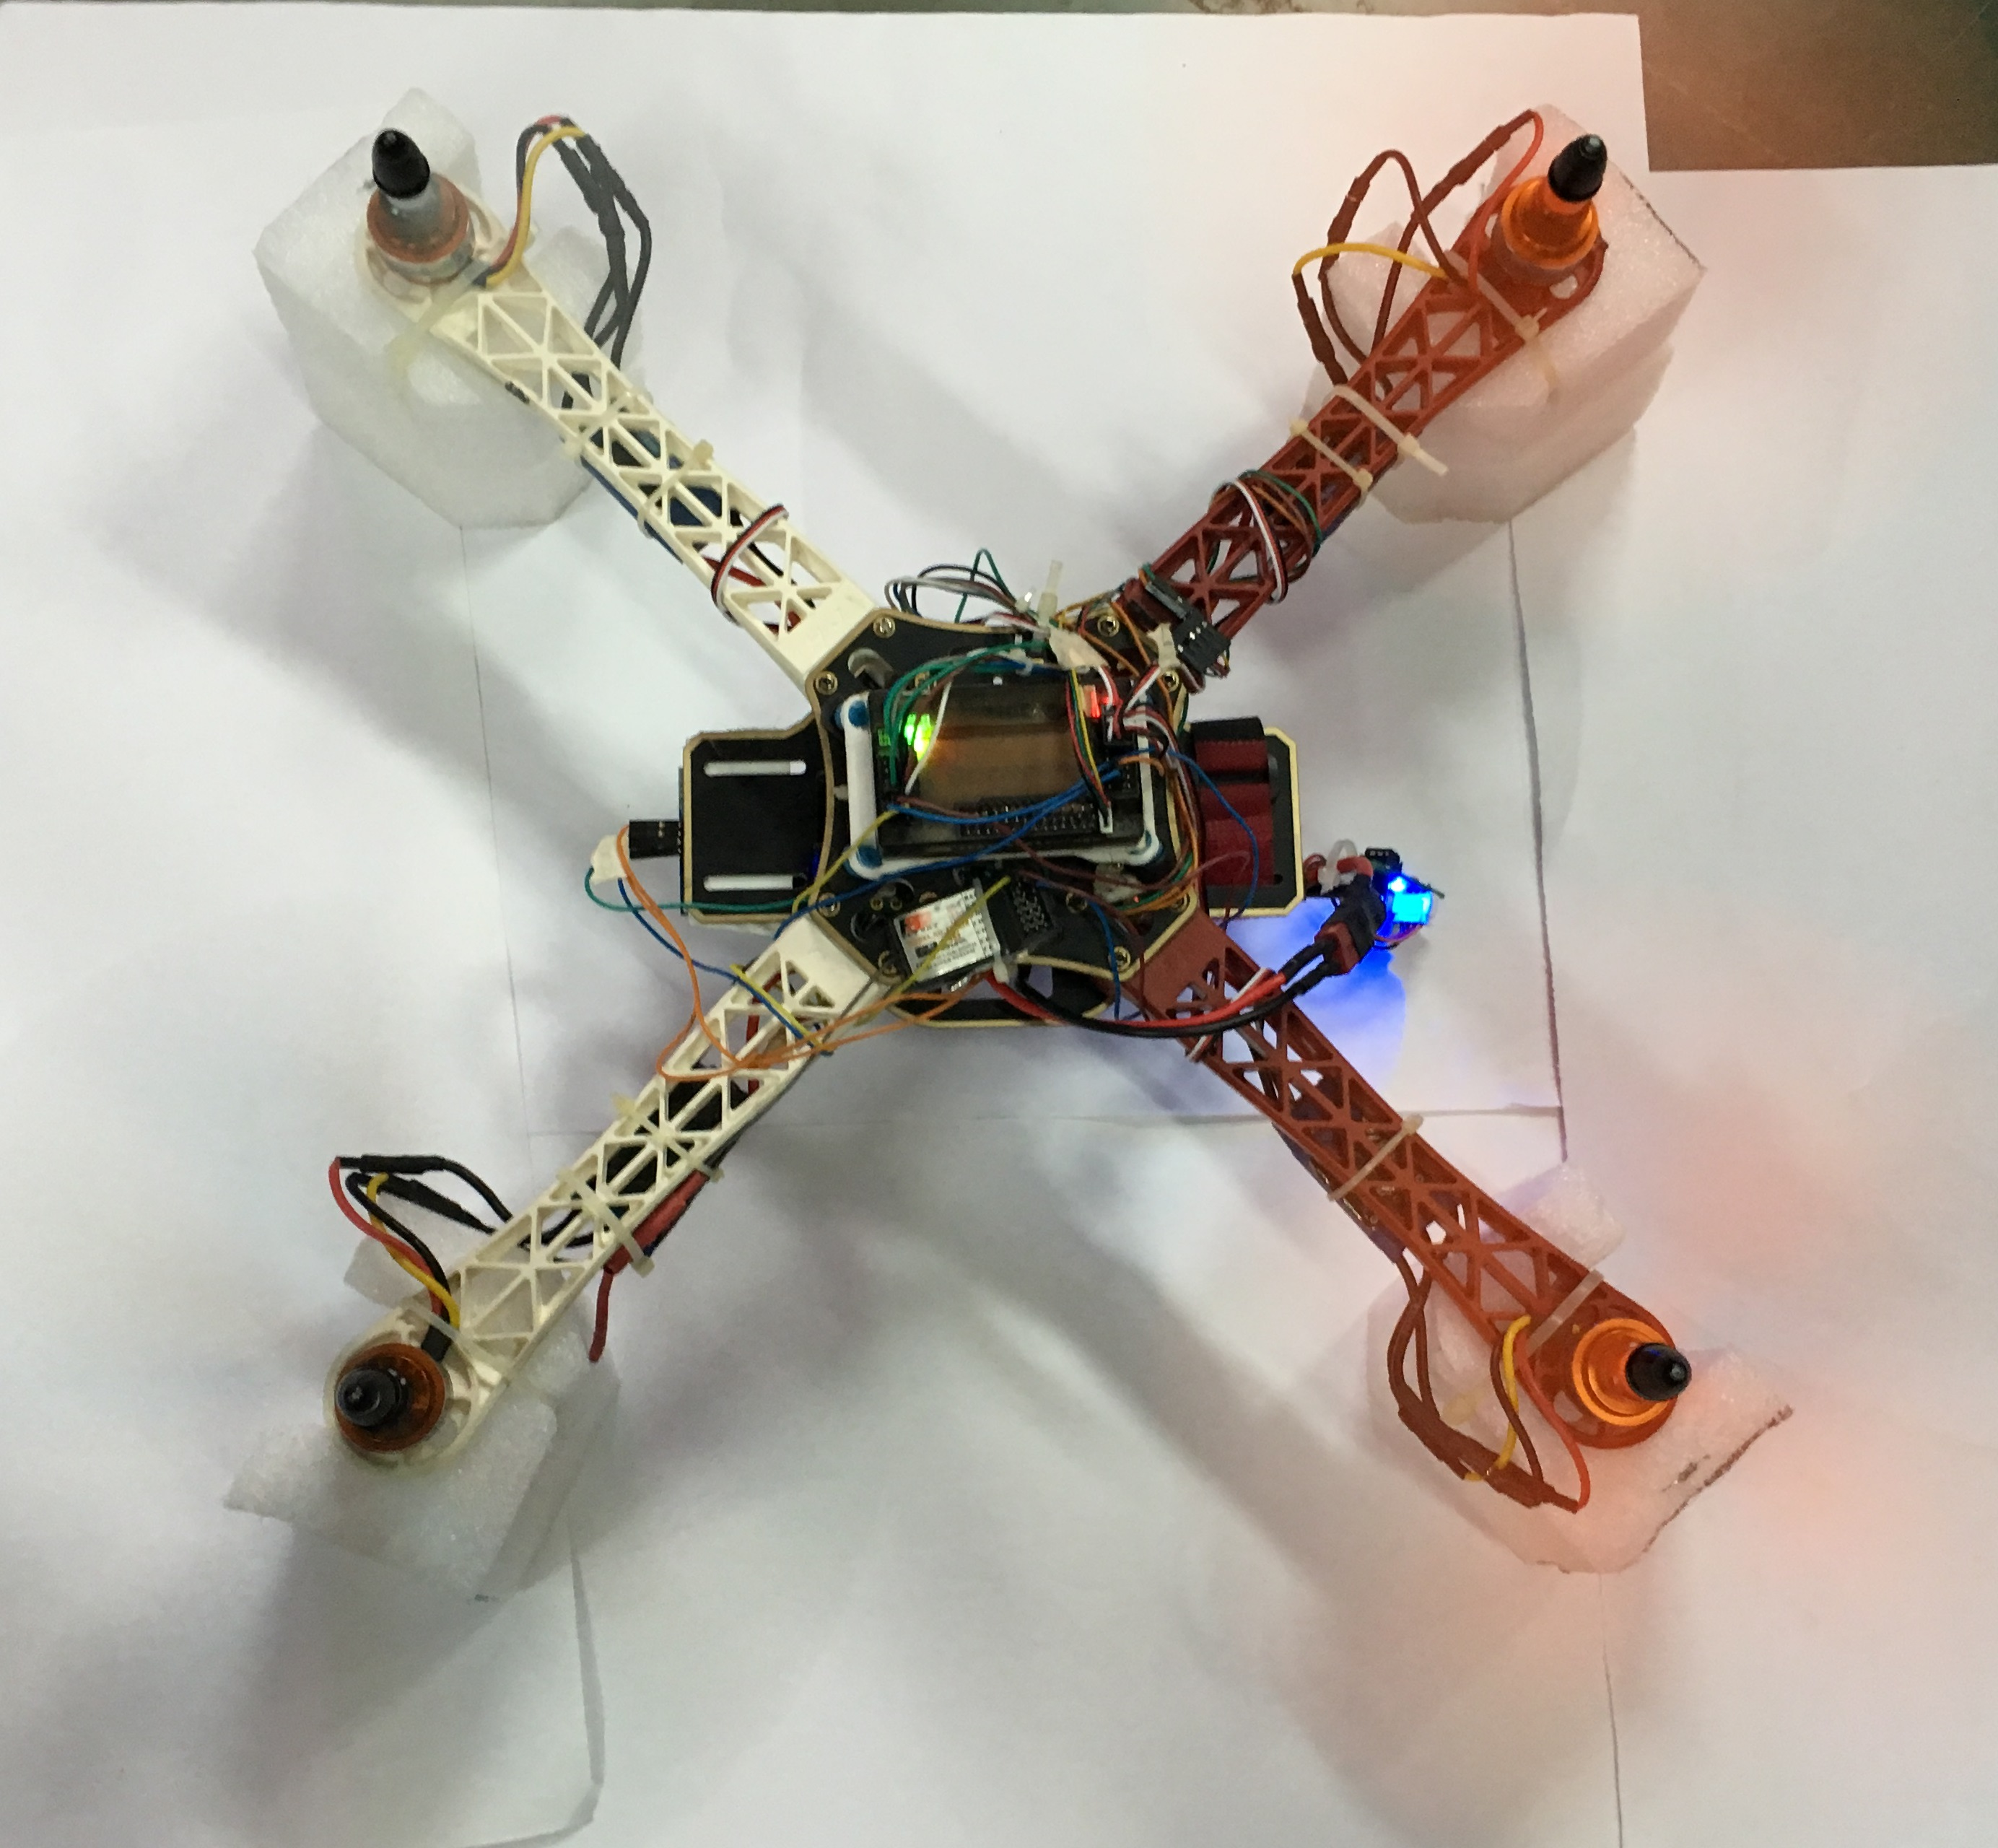
\includegraphics[scale = 0.10]{File_05}}
    \end{figure}
    \\
    \begin{figure}[H]
        \centering
        \fbox{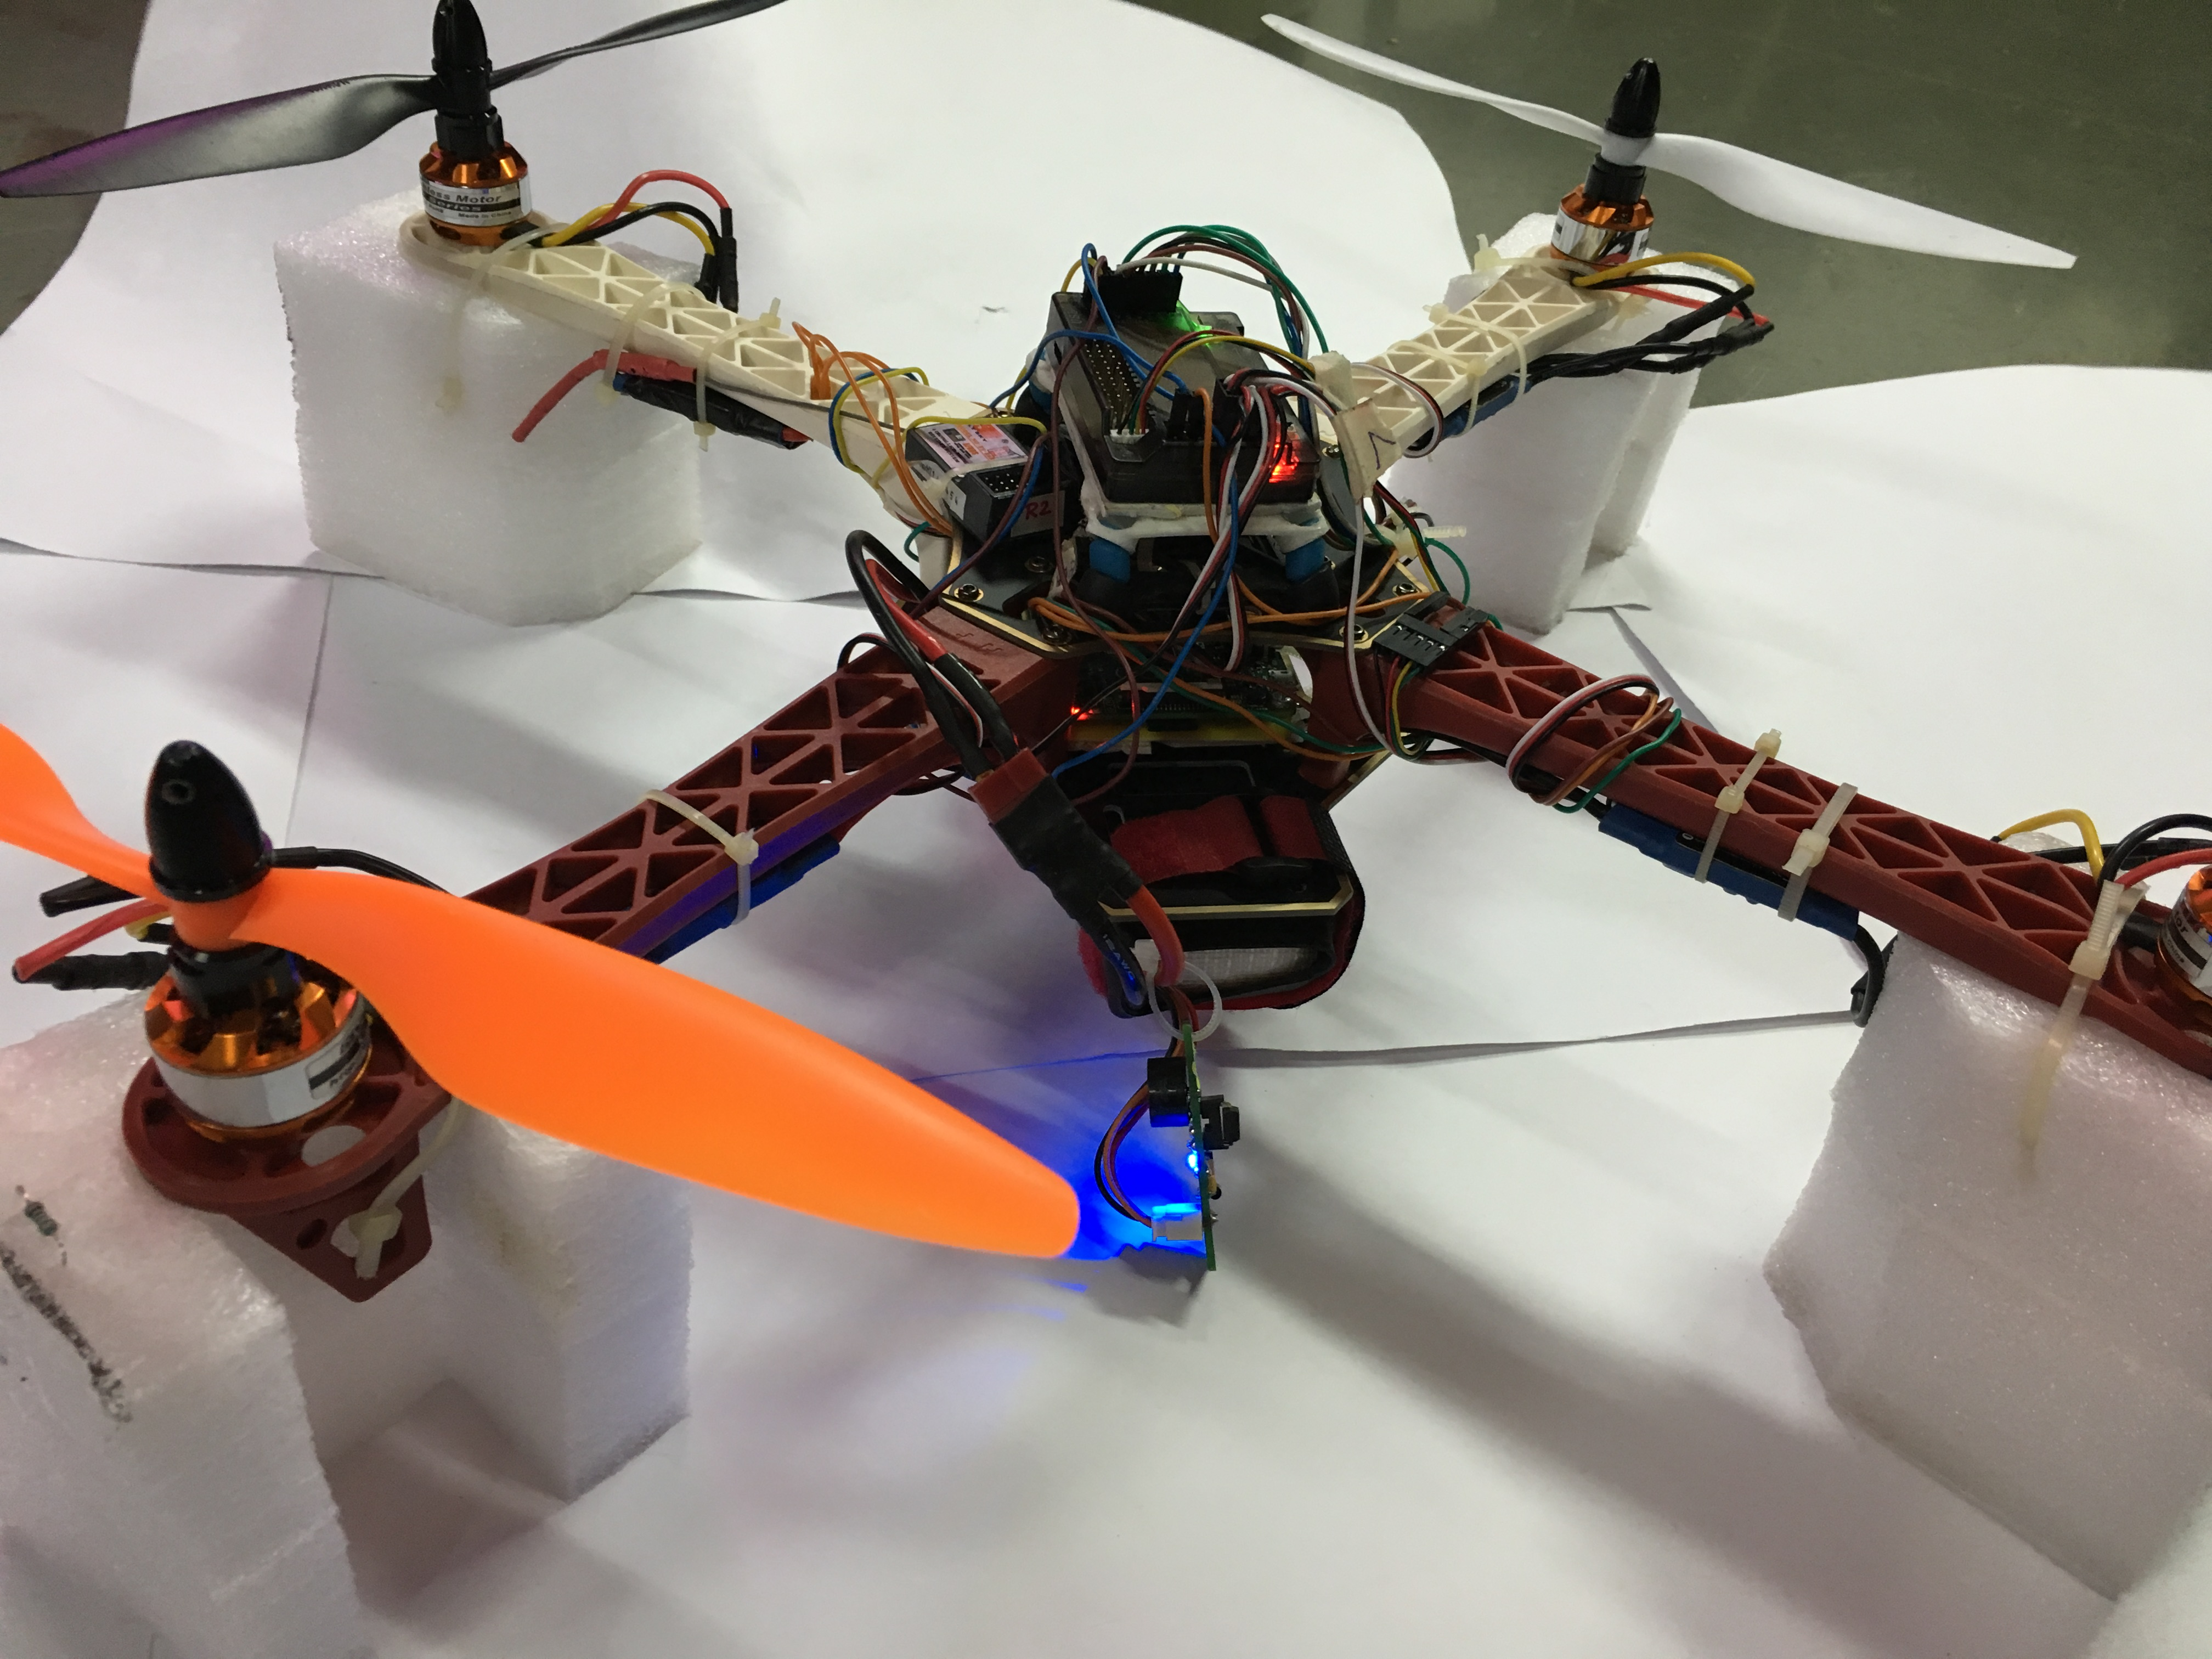
\includegraphics[scale = 0.08]{File_03}}
    \end{figure}
    \textbf{Videos of Flights:}
\begin{enumerate}
    \item \href{https://www.youtube.com/watch?v=oRvV-g8zlzI}{Test flight 1}
    \item \href{https://www.youtube.com/watch?v=dcHOmJOeLvU}{Test flight 2}
    
    \item \href{https://www.youtube.com/watch?v=GHcQYoiWwgk}{Test flight 3}
\end{enumerate}





\section{Future Work}
\begin{enumerate}
    \item Interfacing camera and gimbal
    \item Object tracking drone
    \item Obstacle avoidance
    \item Get GPS data via WiFi and map places
\end{enumerate}

\section{Bug report and Challenges}
Issues with hardware:
\begin{enumerate}
    \item Noise in ultrasonic sensor
    \item Propellers are not balanced
\end{enumerate}
Challenges faced during project:
\begin{enumerate}
    \item Interfacing Raspberry Pi and APM
\end{enumerate}

\section{Refrences}
\begin{enumerate}
    \item \url{http://python.dronekit.io/}
    \item \url{https://discuss.dronekit.io/}
    \item \url{https://github.com/dronekit}
    \item \url{http://ardupilot.org/copter/docs/common-apm25-and-26-overview.html}
    \item \url{http://www.hobbyking.com/hobbyking/store/index.asp}
    \item \url{http://www.rcbazaar.com/default.aspx}
    \item \url{http://www.raspberrypi-spy.co.uk/2012/12/ultrasonic-distance-measurement-using-python-part-1/}
    \item  \url{http://www.modmypi.com/blog/hc-sr04-ultrasonic-range-sensor-on-the-raspberry-pi}
    \item \url{http://ardupilot.org/dev/docs/raspberry-pi-via-mavlink.html}
	\item \url{http://qgroundcontrol.org/mavlink/start}
	\item \url{http://ardupilot.org/copter/docs/common-installing-3dr-ublox-gps-compass-module.html}
	\item \url{http://ardupilot.org/planner/docs/common-install-mission-planner.html}
	\item \url{http://ardupilot.org/planner/docs/common-loading-firmware-onto-pixhawk.html}
	\item \url{http://ardupilot.org/planner/docs/common-connect-mission-planner-autopilot.html}
	\item \url{http://ardupilot.org/copter/docs/connecting-the-apm2.html}
	\item \url{https://multicopterbuild.wordpress.com/how-tos/quadcopter/}
	\item \url{http://dronesforsaleclassified.com/product/dji-hot-wheels-diy-same-paragraph-quadcopter-frame-quality-nylon-f450-v2-rack-integrated-pcb-board-diy-drone-quadrocopter/}
	\item \url{http://www.flyingtech.co.uk/frames-props-parts-accessories/tarot-firefly-450-quadcopter-frame}
	\item \url{http://www.diydrones.com}
	\item \url{http://www.robu.in}
	\item \url{http://www.quadkopters.com}
\end{enumerate}
    
    


\end{document}

